\chapter{Conceptual Design}

\section{Background Research}

The most common water heater is the storage tank water heater. The way it functions is by heating up water that will be stored within a storage tank. This is most conventional since it is easy and cheap to install when comparing it to other water heaters. The limiting factor is that it is limited by the size of the storage tank. It may take a while for the hot water to be heated again if it runs out.

\medskip
Another type of water heater that is used is an Air Source Heat Pump (ASHP). What makes this heat pump unique is that it uses the heat within the air to heat the water. All it needs is a little bit of electricity to power the system. This makes the ASHP two to three times more efficient than most water heaters [4]. The major drawback is that it needs to take heat from the air, therefore it is not suitable for basements or colder climates.

\begin{figure}[ht]
    \centering
    \subfloat[\centering Storage Tank Water Heater {[5]}] {{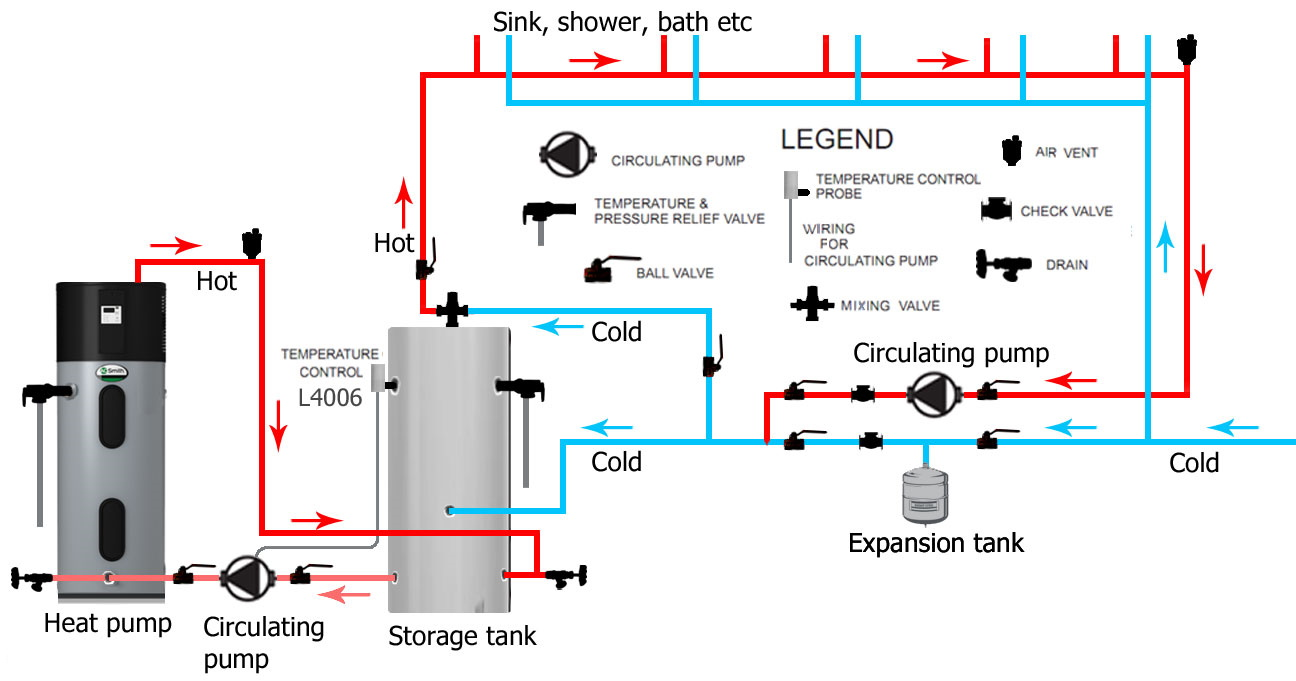
\includegraphics[width=7.7cm]{images/storage_tank_water_heater.jpg}}}
    \qquad
    \subfloat[\centering Air Source Heat Pump Water Heater {[6]}] {{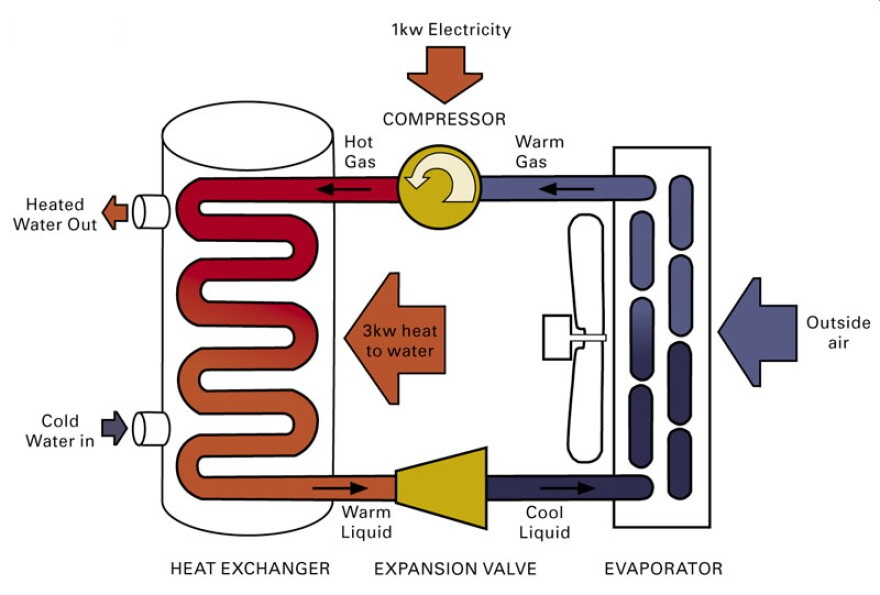
\includegraphics[width=7.7cm]{images/air_source_heat_pump.jpg}}}
    \caption{Conventional Water Heaters}
\end{figure}

\smallskip
Unlike the ASHP, the DX-SAHP uses solar energy to provide the heat needed to heat the water. When comparing Figure 2.2 with Figure 1.1, a solar collector is used instead of an evaporator. This gives all the benefit of an Air Source Heat Pump with the additional benefit of working in colder climates since the sun can provide enough energy to heat the water.

\medskip
When designing a DX-SAHP, it is important to consider the irradiance available in the area. Irradiance is the amount of energy received from the sun within an area. As seen in Table 1, the amount of sun Calgary receives is drastically different between the winter and summer data sets.

\medskip
Winter months are defined from October to March in Table 2.1 while summer is between April to September. The justification behind choosing those date ranges is that it makes use of the entire year, and it is split between when Calgary has the most daylight hours versus the least. It also happens to line up with the solstices.

\medskip

\begin{table}[H]
\centering
\caption{Calgary Irradiance Data}
\rowcolors{2}{gray!20}{white}
\begin{tabular}{|P{10mm}|P{70mm}|P{70mm}|}
    \hline
    \rowcolor{orangeRed}
    Hour &  Average Winter Irradiance Data $(W/m^2)$ & Average Summer Irradiance Data $(W/m^2)$ \\
    \hline
    1 & 0 & 0 \\
    2 & 0 & 0 \\
    3 & 0 & 0 \\
    4 & 0 & 0 \\
    5 & 0 & 1.398907104 \\
    6 & 0 & 12.99453552 \\
    7 & 0.510989011 & 76.3715847 \\
    8 & 7.736263736 & 182.0710383 \\
    9 & 54.40659341 & 327.442623 \\
    10 & 149.6538462 & 445.6065574 \\
    11 & 229.7857143 & 557.2896175 \\
    12 & 289 & 612.0601093 \\
    13 & 316.7087912 & 629.9289617 \\
    14 & 301.6868132 & 587.7923497 \\
    15 & 252.4285714 & 539.8196721 \\
    16 & 178.3241758 & 474.3715847 \\
    17 & 86.85714286 & 374.3879781 \\
    18 & 29.04395604 & 252.4043716 \\
    19 & 3.708791209 & 142.9016393 \\
    20 & 0 & 44.86885246 \\
    21 & 0 & 4.256830601 \\
    22 & 0 & 0 \\
    23 & 0 & 0 \\
    24 & 0 & 0 \\
    \hline
\end{tabular}
\end{table}

\medskip
\section{Collector Design Alternatives}

There are three types of solar collectors that are commonly used in the market; they are flat plate collectors, evacuated tube collectors, and concentrating collectors. Each comes with their own benefits and drawbacks.

\medskip
Flat plate collectors consist of a flat absorber plate that is orientated towards the sun. They use both direct and diffuse solar radiation and normally do not require a tracking system. Their main applications are solar water heating, heating for buildings, air conditioning and heat for industrial processes [7].

\medskip
In contrast, evacuated tube collectors consist of several rows of parallel transparent glass tubes which have the working fluid flowing within it. The glass tubes are cylindrical in shape which results in the sunlight always being perpendicular to the heat absorbing tubes. This is a major benefit since this collector can be used when the sun is low in the sky or on cloudy days and they are particularly useful in colder climates.

\medskip
Concentrating collectors are more suited for systems that require higher temperatures than what is achievable with a flat collector. The concentrating collector can be optimized by decreasing the area of heat loss when comparing it to flat plate collectors. This is done by placing an optical device between the source of radiation and the surface. A disadvantage that this technology has is that a sun tracking system is required to always maximize the incident radiation. This tracking system increases the overall cost of the collector and leads to additional maintenance which is why it was not considered at all for this project [7].

\medskip
When comparing flat plate collectors with evacuated tubes, there are several categories that can be considered. When comparing costs, evacuated tubes are around 10-15\% more expensive than flat plate. This was important to consider due to the limited budget that this project has [8]. Another important area that needs to be looked at would be how the collector can handle snow. Since there will be no tracking system for our design, there will be no way to shake off the snow, so the collector must remove it passively. The benefit of a flat plate collector is that snow can shed easily unlike with evacuated tubes in which it can get stuck due to the tubes creating a strong vacuum [8].

\medskip
Both flat plate and solar collectors are excellent at heating water. The main question that needs to be asked when selecting the collector type is how much water needs to be heated to the desired temperature. Evacuated tubes are great for colder climates since they can heat water up to 121\textdegree C but it has the tendency to overheat. Therefore, evacuated tubes are more commonly used for commercial rather than domestic purposes. Unlike evacuated tubes, flat plate collectors can heat water up to 82\textdegree C which means that it is has smaller chance of overheating. This temperature range is suitable for domestic hot water usage [8].

\medskip
When looking at all the parameters, the flat plate collector was selected instead of the evacuated tube or concentrating collector. Although the evacuated tube collector works better in colder climates than the flat plate collector, it was excessive in terms of both cost and design work for domestic water heating. The flat plate satisfies many requirements for a collector in colder climates, and it is the recommended collector for domestic water heating [8]. Therefore, for the design, the flat plate collector was chosen.

\section{Refrigerant Alternatives}

A refrigerant is a working fluid used in the thermodynamic cycle of a heat-pump, where the fluid will undergo multiple phase changes from liquid to vapor and vice versa, throughout the system cycle. One of the first components in a heat pump, which must be determined early on, is the refrigerant. To determine which components (i.e., compressor, condenser, and expansion valve) will be used in the DX-SAHP, the working fluid must be selected, and calculations will be performed to find the operating points of the system. Although there are many refrigerants to choose from, the list can be drastically cut down depending on multiple criteria. These criteria will look at the environmental acceptability, safety, application, performance, and the economics associated with various refrigerants.

\medskip
The Ozone Depletion Potential (ODP) is a measure of a refrigerant’s ability to damage the ozone layer relative to CFC-11 with an ODP of 1. Emissions from CFC’s (chlorofluorocarbons), HCFC’s (hydrochlorofluorocarbons), and other synthetic chemicals which created an “ozone hole” over the South Pole [9] have led to the Montreal Protocol on Substances that deplete the Ozone layer [10] – a global agreement made to phase out ozone-depleting substances. For the DX-SAHP, only refrigerants with an ODP equal to zero will be considered.

\medskip
The Global Warming Potential (GWP) is the next major criterion regarding environmental acceptability. This is a metric measuring the energy of emissions, which one ton of a specific gas will absorb relative to the emissions of one ton of carbon dioxide (\ch{CO2}) over a hundred-year period [11]. For example, a refrigerant with a GWP of 2088 will have 2088 times the global warming potential of \ch{CO2} over 100 years. In 2016, the Kigali amendment was made to the Montreal Protocol [12], proposing a complete phase down of HFCs by 2047 due to their high global warming potential. Furthermore, the European Union [13] took action to place market prohibitions on gases with a GWP greater than 750 in air-conditioning systems by 2025. Therefore, the refrigerants in the selection will also be required to have a GWP below 750.

\medskip
Refrigeration cycles have three distinct applications: high temperature (comfort conditioning), medium temperature (food refrigeration), and low temperature (transport refrigeration). Domestic water heating falls into high temperature comfort conditioning applications. The most widely used refrigerant in these applications has been R-410A. Due to the high SEER (Seasonal Energy Efficiency Ratio) ratings R-410A has provided with many heat pump systems as compared to other refrigerants, it has dominated the air conditioning market for components. However, due to R-410A’s high GWP of 2088, refrigerants with similar thermodynamic properties used as replacements for the eventual phase down of R-410A were explored.

\newpage
Following the ASHRAE Standard 34 refrigerant safety classification, most refrigerants in use currently pose a very low toxicity and flammability threat – giving an ASHRAE safety designation of A1. Following the ASHRAE Standard 34 [14] refrigerant safety classification, most refrigerants in use currently pose a very low toxicity and flammability threat – giving an ASHRAE safety designation of A1. ASHRAE Standard 34 assigns refrigerants to two toxicity (A or B), and four flammability classes (1, 2, 2L, 3). The safety designations for refrigerants are as follows:

\begin{itemize}[itemsep=3mm, parsep=-1mm]
\item Class A (Low Toxicity)
    \begin{itemize}
        \item Occupational exposure limit is 400ppm or greater
    \end{itemize}
\item Class B (High Toxicity)
    \begin{itemize}
        \item Occupational exposure limit is less than 400ppm.
    \end{itemize}
\item Class 1 (No flame propagation)
    \begin{itemize}
        \item No flame propagation at 60\textdegree C and atmospheric pressure.
    \end{itemize}
\item Class 2L (Low flammability)
    \begin{itemize}
        \item Flame propagation at 60\textdegree C and atmospheric pressure.
        \item Lower Flammability Limit $> 0.10kg/m^3$ and Heat of Combustion $< 19,000 kJ/kg$
        \item Burning velocity <= 10cm/s at 23\textdegree C
    \end{itemize}
\item Class 2 (Flammable)
    \begin{itemize}
        \item Flame propagation at 60\textdegree C and atmospheric pressure.
        \item Lower Flammability Limit $> 0.10kg/m^3$ and Heat of Combustion $< 19,000 kJ/kg$
    \end{itemize}
\item Class 3 (High flammability)
    \begin{itemize}
        \item Flame propagation at 60\textdegree C and atmospheric pressure.
        \item Lower Flammability Limit $<= 0.10kg/m^3$ or Heat of Combustion $< 19,000 kJ/kg$
    \end{itemize}
\end{itemize}

\medskip
Because the system is being designed for a residential water heating supply, due to possibility of leakage, only refrigerants designated in Class A toxicity will be used.

\medskip
As with many design considerations in engineering, there is an equivalent exchange when reducing the global warming potential of refrigerants. A general trend can be observed in refrigerants where a lower GWP equates to a higher flammability designation; most new generation refrigerants with a GWP less than 750 have an ASHRAE safety designation of A2L. While refrigerants of Class 1 are the most desirable, Class 2L refrigerants can also be considered safe [15] to use in domestic heating systems as they have a high Minimum Ignition Energy and would need to be exposed to an open flame or high energy source with sufficient concentrations to ignite.

\medskip
Although each refrigerant will result in different system efficiencies, by looking at the critical temperature of the refrigerant, a correlation can be made for both the coefficient of performance and the cooling capacity of the system. As the critical temperature of the refrigerant increases, the coefficient of performance of the system is found to increase, while the cooling capacity is found to decrease [16]. A higher coefficient of performance will ultimately result in a lower energy bill for the end user, while a lower cooling capacity will result in a larger system. As the project location is for a cold climate in Calgary, the refrigerant must also be chosen to have a freezing point, $T_{fp} < \SI{-50}{\celsius}$. Furthermore, CoolProp [17] was used to conduct the thermodynamic analysis, and therefore, refrigerants of choice must be available on the database such that the system calculations can be performed.

\medskip
Finally, the economics and procurement of the refrigerants will be considered where the system will require between 1-5kg of charge. After contacting vendors, many refrigerants were found to have more than 3 months lead times due to COVID-19 supply chain issues, and as a result would not satisfy the project’s timeline. Many new generation refrigerants were also found to be cost-ineffective when compared to their incremental performance benefits. These refrigerants ranged from \$400 to \$3000 per their minimum selling quantities.

\medskip
A design requirements table was then created to easily compare the refrigerants as seen below.

\medskip
\begin{table}[H]
\centering
\caption{Refrigerant Criteria}
\rowcolors{2}{gray!20}{white}
\begin{tabular}{|P{23mm}|P{23mm}|P{23mm}|P{23mm}|P{23mm}|P{23mm}|}
    \hline
    \rowcolor{orangeRed}
    Refrigerant &  ODP & GWP & Alternative To & Safety Class & $T_{critical}$ (\textdegree C) \\
    \hline
    R-410A           & 0 & 2088 & R-22   & A1  & 72.13 \\
    R-717 (\ch{NH3}) & 0 & 0    & R-22   & B1  & 132.4 \\
    R-1234yf         & 0 & 4    & R-134A & A2L & 94.70 \\
    R-1234ze         & 0 & 1    & R-134A & A2L & 109.4 \\
    R-32             & 0 & 675  & R-410A & A2L & 78.40 \\
    R-454B           & 0 & 466  & R-410A & A2L & 78.10 \\
    R-454C           & 0 & 148  & R-410A & A2L & 82.40 \\
    R-455A           & 0 & 146  & R-410A & A2L & 86.60 \\
    R-466A           & 0 & 733  & R-410A & A1  & 76.50 \\
    R-515B           & 0 & 299  & R-134A & A1  & 108.7 \\
    R-290            & 0 & 3    & R-410A & A3  & 97.00 \\

    \hline
\end{tabular}
\end{table}

\medskip
After assessing the criteria of each refrigerant, and contacting vendors of the remaining options, it was determined that R-32 was to be the refrigerant of choice in the DX-SAHP. The decision was contingent upon the refrigerant’s suitability with the team’s initial selection criteria. With a zero ODP, a GWP less than 750, a critical temperature of 78.4\textdegree C, but most importantly, a procurement time of 2 months, the R-32 was determined to be the appropriate working fluid.

\medskip
Upon determination of R-32 as the working fluid for the system, the component matching phase began. Although some components were found for this refrigerant (e.g., expansion valve), when looking for a compressor compatible with R-32, and which could be procured within a reasonable time frame, component matching proved to be difficult.

\medskip
After consulting with a subject matter expert working in the heating ventilation and cooling (HVAC) sector for over 15 years, the team determined the reason for the difficulties to be that R-32 and all other similar new generation refrigerants are still considered novel to the industry. As R-410A is still dominating the air conditioning industry in North America, components for comfort cooling heat pump applications are designed around R-410A being the working fluid. However, the research was not in vain; since R-32 is the widespread refrigerant of choice in Asia and is slowly being phased in around parts of Europe as the next replacement for R-410A, it is beneficial to have considered it as a potential working fluid for the DX-SAHP.

\medskip
Finally, although the GWP was far too high, it was still suggested to design the system using R-410A as North America has not yet caught up with the refrigerant phase down plan. Furthermore, the use of R-410A as a system refrigerant is not detrimental to the project’s environmental considerations as the final solution to avoid the use of a high GWP refrigerant is through sourcing drop-in replacements. A drop-in replacement for R-410A (such as R-470A) is a refrigerant which can simply swap R-410A while maintaining the same system components. This allows for the system calculations, and thus, the system components to be modeled and procured based upon R-410A as the working fluid. The advantage of taking the approach of using drop-in refrigerants is that, as new refrigerants become available, supply chain delays would not hinder the progress of the build assembly as R-410A could always be used to complete the project.

\section{Component Design Alternatives}

\subsection{Compressor Type Selection}

For the purposes of the compressor in the DX-SAHP, the hermetic sealed variable speed compressor has been selected as the primary choice. These types of compressors are positive displacement and can achieve higher compression ratios per single stage of compression [18]. They are more compact and less prone to vibration issues.

\medskip
Hermetic compressors are widely used in domestic refrigeration systems where continuous maintenance cannot be ensured by the user. A hermetic compressor consists of the compressor being mounted directly on the shaft of the motor. The compressor and motor are confined together within an outer shell, reducing the potential for dust particles to enter as easily, and thereby reducing any impact on the operation of the compressor [19]. With both the compressor and motor being directly coupled on the same shaft and confined within a common casing, the potential for leakage of R-410A is reduced and essentially eliminated [20]. The investigated hermetic compressors for the purposes of system analysis are of the reciprocating and rotary types.

\medskip
The variable speed aspect of the compressor works by adjusting the speed of the motor to meet required demands while conserving energy in the process. For the purposes of this analysis, having the ability to control the speed of the compressor allows for the control of the pressure differential of refrigerant, R-410A. Therefore, it is essential to control the varying inlet conditions entering the compressor to obtain a condensation temperature of 60\textdegree C.

\medskip
The advantages of a hermetic variable speed compressor are less noise, faster pull-downs to our established condensation temperature, more consistent temperature, less wear on system components, less vibrations, and decreased energy bills [21]. The disadvantage of using this type is that the motor drive cannot be maintained in its place and if the motor were to fail, the whole compressor would need to be replaced.

\medskip
Out of the many available compressors, the following design alternatives for a hermetic variable speed compressor have been taken into consideration, allowing for use in domestic water heating applications [22] [23].

\medskip
\begin{enumerate}[itemsep=3mm, parsep=-1mm]
    \item Scroll variable speed compressor [24]
    \item Reciprocating variable speed compressor [25]
    \item Rotary screw variable speed compressor
    \item Centrifugal variable speed compressor
    \item Open motor hermetic speed compressor
\end{enumerate}

\medskip
The following figure shows common compressors and their classification.

\medskip
\begin{figure}[ht]
    \centering
    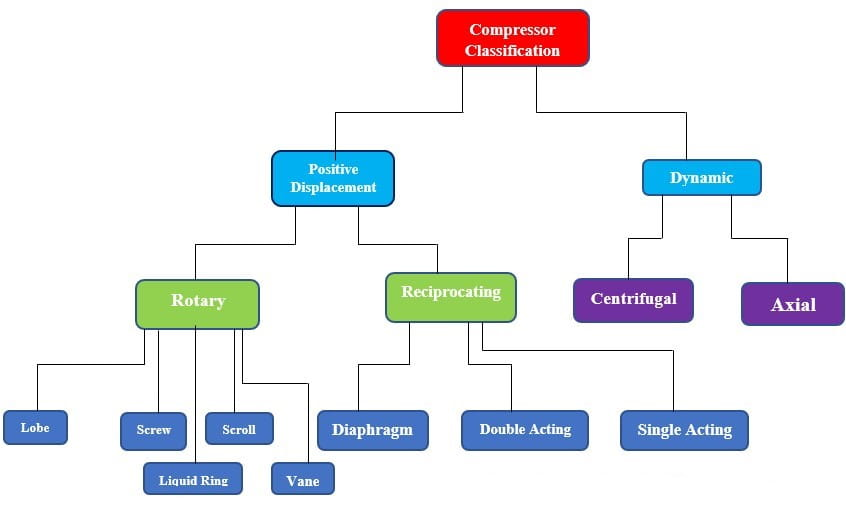
\includegraphics[width=\textwidth]{images/compressor_types.jpg}
    \caption{Compressor Classification}
\end{figure}

\medskip
Out of the above five listed compressors, the primary design alternative would be the scroll variable speed compressor. The rotary screw and reciprocating positive displacement variable speed compressors may also be used for the purposes of the DX-SAHP. However, since rotary screw variable speed compressors are more commonly used in commercial and industrial applications, they will not be considered as the primary design alternative. The reciprocating variable speed compressors are commonly used in residential applications except that this type does not operate as type rotary which is preferred for the analysis of DX-SAHP. Scroll variable speed compressors are available for lower power ratings, are compatible with R-410A, come in a single phase, and can operate within the operating pressures of the system. They exhibit energy saving capabilities [27] [28].

\medskip
The reasons for not selecting the remaining as design alternatives is because while all the above can be used in similar applications, the centrifugal type compressors are often used in applications such as, large chillers, refineries, plants, and industrial applications [29]. Therefore, they operate with higher horsepower and for higher operating pressures than required for the purpose of the DX-SAHP. Additionally, centrifugal compressors consist of dynamic applications whereas for the purposes of the system, a positive displacement compressor shall be used. The open motor variable speed hermetic compressor is not suitable as it has a higher potential of refrigerant leakage than a sealed hermetic variable speed compressor would.

\subsection{Condenser Type Selection}

Storage tank water heaters are by far the most prevalent configuration of water heaters available on the market today; however, tankless or “On-Demand” water heaters are slowly acquiring some of that market share due to their reputation of running more efficiently. For the purposes of selecting a condenser/water storage tank for the Direct Expansion Solar Assisted Heat Pump, the team considered the following factors:

\medskip
\begin{enumerate}[itemsep=3mm, parsep=-1mm, label=\roman*.]
    \item The operational time span of the evaporator/collector.
    \item The stability of meteorological conditions of the design locale.
    \item The temperature of the inlet municipal water supplied for domestic use.
\end{enumerate}

\medskip
By relying on weather station data from the Government of Canada [30], we determined the average, daily “bright sunshine hours”, to be 4.68 hours for Calgary during the winter season. These hours would support peak operation of the Solar Thermal Collector, and outside of which, the system performance may decline, and in extreme conditions, stagnate, ceasing the supply of hot domestic water in the absence of a suitable thermal mass. Assessing the stability or consistency of the meteorological conditions, such as ambient temperatures and average irradiance, the team concluded that the short operational time frame, paired with the instability of meteorological conditions and potential for inclement winter weather conditions, such as extreme subzero temperatures and collector shading due to snowfall, the DX-SAHP cannot support a tankless water heater module as a steady supply of hot water would not be guaranteed outside of optimal operational conditions. Furthermore, considering that the temperature of the supplied groundwater determines the length of the heating period in a tankless water heater, and that inlet municipal water is supplied at approximately 10\textdegree C during the winter, adopting a tankless water heater is not a feasible option for this application due to prolonged heating times. In conclusion, the team opted to adopt a shell and coil condenser wherein the shell or “storage tank” would serve as the water reservoir or thermal mass from which emergency supply of hot water could be provisioned. Further selection considerations are highlighted in section 3.3.2 below.

\subsection{Expansion Valve Selection}

For the purposes of the throttling valve in the DX-SAHP system, an electronic expansion valve was selected. Throttling valves allow control of the amount of mass flow rate by adjusting the size of the flow path through the valve. The two types that were initially compared were the thermostatic valve (TXV) and the electronic expansion valve (EXV). The following explanation tends to the operation of both [31], differences [32], and final selection choice.

\medskip
TXV’s typically use sensing bulbs to sense the temperature of the suction line. These bulbs are slightly warmer than the saturation temperature of the refrigerant and have an increase in pressure when the suction line temperature exceeds the saturation temperature. The increased pressure in the bulb indicates that more refrigerant is required to manage the system’s evaporating heat load. The opening of the valve occurs by the internal connections from the bulb to the power element. The power element consists of a diaphragm and with increasing pressure, the diaphragm is bent downwards to open the valve.

\medskip
EXV’s use an electronic controller to calculate the superheat based on the temperature and pressure at the suction line, and the outlet of the solar flat plate collector. For the controller to read the pressure and temperatures, respectively, pressure transducers and thermistors may be used. The programming of the controller controls the valve movement by either opening or closing the valve, based on the inputs read by the sensors.

\medskip
The main disadvantages of using a TXV is that if the pressure differential between the sensing bulb, combined pressure below the diaphragm, and the spring are significantly reduced, the opening and closing of the valve will be affected. Ultimately, this creates a problem for the system to operate as efficiently, mainly on the release of the mass flow rate as required for the heating load.

\medskip
Based on this, the EXV was selected as the throttling valve to be placed in the system. EXV’s offer more flexibility for system design requirements by having the ability to use the controller without needing to physically adjust the valve.